\documentclass[12pt,oneside]{uhthesis}
\usepackage{subfigure}
\usepackage[ruled,lined,linesnumbered,titlenumbered,algochapter,spanish,onelanguage]{algorithm2e}
\usepackage{amsmath}
\usepackage{amssymb}
\usepackage{amsbsy}
\usepackage{caption,booktabs}
\captionsetup{ justification = centering }
%\usepackage{mathpazo}
\usepackage{float}
\setlength{\marginparwidth}{2cm}
\usepackage{todonotes}
\usepackage{listings}
\usepackage{xcolor}
\usepackage{multicol}
\usepackage{graphicx}
\floatstyle{plaintop}
\restylefloat{table}
\addbibresource{Bibliography.bib}
% \setlength{\parskip}{\baselineskip}%
\renewcommand{\tablename}{Tabla}
\renewcommand{\listalgorithmcfname}{Índice de Algoritmos}
%\dontprintsemicolon
\SetAlgoNoEnd

\definecolor{codegreen}{rgb}{0,0.6,0}
\definecolor{codegray}{rgb}{0.5,0.5,0.5}
\definecolor{codepurple}{rgb}{0.58,0,0.82}
\definecolor{backcolour}{rgb}{0.95,0.95,0.92}

\lstdefinestyle{mystyle}{
    backgroundcolor=\color{backcolour},   
    commentstyle=\color{codegreen},
    keywordstyle=\color{purple},
    numberstyle=\tiny\color{codegray},
    stringstyle=\color{codepurple},
    basicstyle=\ttfamily\footnotesize,
    breakatwhitespace=false,         
    breaklines=true,                 
    captionpos=b,                    
    keepspaces=true,                 
    numbers=left,                    
    numbersep=5pt,                  
    showspaces=false,                
    showstringspaces=false,
    showtabs=false,                  
    tabsize=6
}

\lstset{style=mystyle}

\title{Título de la tesis}
\author{\\\vspace{0.25cm}Nombre del autor}
\advisor{\\\vspace{0.25cm}Nombre del primer tutor\\\vspace{0.2cm}Nombre del segundo tutor}
\degree{Licenciado en (Matemática o Ciencia de la Computación)}
\faculty{Facultad de Matemática y Computación}
\date{Fecha\\\vspace{0.25cm}\href{https://github.com/username/repo}{github.com/username/repo}}
\logo{Graphics/uhlogo}
\makenomenclature

\renewcommand{\vec}[1]{\boldsymbol{#1}}
\newcommand{\diff}[1]{\ensuremath{\mathrm{d}#1}}
\newcommand{\me}[1]{\mathrm{e}^{#1}}
\newcommand{\pf}{\mathfrak{p}}
\newcommand{\qf}{\mathfrak{q}}
%\newcommand{\kf}{\mathfrak{k}}
\newcommand{\kt}{\mathtt{k}}
\newcommand{\mf}{\mathfrak{m}}
\newcommand{\hf}{\mathfrak{h}}
\newcommand{\fac}{\mathrm{fac}}
\newcommand{\maxx}[1]{\max\left\{ #1 \right\} }
\newcommand{\minn}[1]{\min\left\{ #1 \right\} }
\newcommand{\lldpcf}{1.25}
\newcommand{\nnorm}[1]{\left\lvert #1 \right\rvert }
\renewcommand{\lstlistingname}{Ejemplo de código}
\renewcommand{\lstlistlistingname}{Ejemplos de código}

\begin{document}

\frontmatter
\maketitle

\begin{dedication}
    Dedicación
\end{dedication}
\begin{acknowledgements}
    Queridos padres, hermana, esposa, amigos y todos aquellos que han sido parte esencial de mi trayectoria académica,

    En este momento de culminación, quiero expresar mi más profundo agradecimiento a cada uno de ustedes por 
    su apoyo incondicional, amor y presencia constante a lo largo de mi camino. Vuestras contribuciones han 
    sido fundamentales para mi éxito y desarrollo personal, y les dedico mis más sinceros agradecimientos.

    Padres, no encuentro palabras suficientes para expresar mi gratitud por las enseñanzas que me 
    han brindado. Desde el comienzo, han sido mi faro en la oscuridad, guiándome con su sabiduría y amor. Vuestra 
    paciencia, sacrificio y confianza en mí han sido los pilares que me han mantenido en pie durante los 
    desafíos que la vida me ha presentado. Gracias por creer en mis capacidades y por brindarme todas las herramientas 
    necesarias para alcanzar mis metas. Sin su amor incondicional, nada de esto hubiera sido posible.

    Agradecer a mi hermana Elena, por su alegría infinita que contagia a todo ser a su alrededor, por los consejos
    y experiencias brindadas en todos estos años de vida y, por darme la satisfacción, de saber que el único ser humano
    que me acompañó y me acompañará durante mi estancia en el universo es la mejor persona que he conocido.

    A Brenda, mi compañera de vida. Tu amor sin barreras, tu felicidad, 
    comprensión y apoyo me han dado la fortaleza para superar los obstáculos y perseverar en mi camino. 
    Las palabras de aliento y tu presencia constante han sido mi mayor motivación. Gracias por comprender 
    mis largas horas de estudio, por celebrar mis triunfos y por secar mis lágrimas en los momentos de 
    dificultad. Eres mi inspiración y mi mayor alegría.

    Amigos, ustedes han sido mi refugio en los momentos de estrés y felicidad en los momentos de 
    triunfo. Vuestra amistad ha sido un regalo invaluable; los días de estudios, las reuniones en casa de 
    Jorge y las burlas constantes me las llevaré a la tumba. Gracias por estar a mi lado, 
    por escucharme, comprenderme y brindarme vuestro apoyo.

    A mis profesores y mentores, en especial a mi tutora, Aymée. Vuestra sabiduría y dedicación han 
    sido un motor de conocimiento en mi camino académico. Gracias por compartir vuestro saber, por 
    desafiarme a ir más allá de mis límites y por alentarme a seguir aprendiendo. Vuestras enseñanzas, 
    correcciones y orientación han sido fundamentales para mi crecimiento y desarrollo. Agradezco 
    sinceramente el tiempo y el compromiso que han invertido en mi formación.
\end{acknowledgements}
\begin{opinion}
    El trabajo de diploma Simulación computacional para la dinámica de enfermedades transmitidas por vectores, presentado por el estudiante Ernesto Alfonso Hernández, para optar por el título de licenciado en Ciencia de la Computación, se corresponde con intereses del grupo de Modelación Biomatemática de la facultad de Matemática y Computación que trabajamos la modelación, solución y análisis de problemas aplicados a las biociencias.

Cuando hice propuestas para temas de diploma, entre mis aspiraciones estaba lograr resultados manejables para enfermedades trasmisibles utilizando redes complejas, ya que me pareció alentador lo aprendido a través de un trabajo anterior, de hace ya algunos años con una diplomante de la carrera de Matemática. El entusiasmo de Ernesto, ante estas alternativas, me ilusionó y desde el primer encuentro me pareció que tenía claro cómo trabajar.

Para lograr los objetivos que nos propusimos y que este trabajó superó, el diplomante realizó una investigación con el objetivo de implementar un modelo basado en redes complejas para simular la dinámica de transmisión del dengue entre personas y vectores en un determinado entorno, a través de la simulación computacional. Vale aclarar que hablamos de dengue, por las tareas en que el Grupo de Investigación está involucrado, pero que lo presentado es perfectamente válido para cualquier enfermedad transmitida por vectores.

Los que han participado en las defensas de otros trabajos que he dirigido, saben que por lo general repito que los estudiantes han trabajado con mucha independencia (especialmente con estudiantes de computación, pues mis conocimientos y posibilidades en temas de programación son muy limitados) y esta vez, tendré que repetirme pero además, con creces. 

Debo confesar que los pasos para lograr los objetivos específicos y que incluyeron el estudio y la comparación de modelos existentes para la simulación de epidemias, la selección y diseño de un modelo que representara a las personas como agentes, la implementación de una aplicación que simulara diferentes escenarios y permitiera la validación del modelo desarrollado, fueron trazados y transitados por Ernesto con una lógica incuestionable.

Y como si la estrategia diseñada no fuera ya en sí competente, Ernesto, gracias a estudios independientes y muy actuales, me propuso trabajar con mapas cognitivos difusos que representan las acciones como conjuntos difusos, lo que permitió que los agentes tuviera opciones de decisión para sus acciones, en función de su percepción del medio.

Además de este trabajo con importantes novedades teóricas y conceptuales, que por supuesto, requieren de conocimientos que no están contenidos en las asignaturas del currículo de la carrera, me toca agradecer la creación de una aplicación de escritorio para facilitar la manipulación y visualización del modelo desarrollado, con posibilidades de variantes que puede manejar el usuario. 

Como afirma el propio autor en la Introducción de su trabajo, esta investigación realiza una contribución significativa al campo de la simulación de epidemias, con resultados que demuestran la validez de los modelos basados en agentes y pudiera convertirse en una herramienta para los decisores de Salud en nuestro país.

Ha sido y lo sabemos, poco el tiempo con que han contado los diplomantes en este atípico último año de su carrera, para concluir sus trabajos de tesis, por ende, valoro doblemente los resultados obtenidos.

Considero que el trabajo presentado cumple con creces los requerimientos para ser defendido como tesis de licenciatura, con una evaluación excelente. Quería destacar de manera adicional, que me ha sorprendido muy favorablemente la maestría para escribir y redactar de Ernesto. 

Toda obra humana es perfectible y por supuesto que hay mucho que perfeccionar para que esta herramienta cumpla con mayores expectativas, pero estoy segura, porque lo ha demostrado sin lugar a dudas, que Ernesto tiene capacidad y condiciones para empeños mayores.

Por mi parte, lo invito a que mantengamos el mismo intercambio ameno y fructífero para dar continuidad al mismo y a trabajos futuros.

Le agradezco el trabajo conjunto, le deseo grandes éxitos en su vida profesional y lo felicito de corazón.

\begin{tabular}{r l}
    
\includegraphics[width=0.2\linewidth]{Graphics/Opinion_Firma.png}\\
    \hrulefill \\
    Dra. Aymée Marrero Severo\\                    
    Tutora                                                        
\end{tabular}



\end{opinion}
\begin{resumen}
	En el presente trabajo, se realizó una investigación con el objetivo de implementar 
    un modelo basado en redes complejas para simular la dinámica de personas y vectores 
    en un entorno. Los objetivos específicos incluyeron el estudio y la comparación de 
    modelos existentes para la simulación de epidemias, el diseño de un modelo que 
    representara a las personas como agentes, la implementación de una aplicación que 
    permitiera simular diferentes escenarios y la validación del modelo desarrollado.

    En este estudio, se logró simular el comportamiento de las personas en la sociedad actual 
    al representar sus principales acciones en el modelo. Además, se modeló el entorno de 
    convivencia como una red compleja, donde las relaciones entre las personas se 
    representaron mediante aristas en un grafo. Estos logros cumplen con el objetivo general 
    de la investigación. También, se modeló a las personas como agentes para analizar su toma 
    de decisiones. Se desarrolló un Mapa Cognitivo Difuso que representa a las acciones como 
    conjuntos difusos, lo que permitió que los agentes decidieran entre diferentes acciones 
    en función de sus sentimientos y el grado de pertenencia a los conjuntos.

    Adicionalmente, se creó una aplicación de escritorio para facilitar la manipulación y 
    visualización del modelo desarrollado, permitiendo realizar simulaciones con los valores 
    de los parámetros que el usuario entienda. Los resultados fueron validados 
    utilizando estadísticas de trabajos previos relacionados con la simulación de epidemias, 
    lo que respalda la solidez de los resultados obtenidos y el cumplimiento de los objetivos 
    específicos propuestos.

    Esta investigación realiza una contribución significativa al campo de la simulación de 
    epidemias. Los resultados demuestran la utilidad de los modelos basados en 
    agentes para simular este tipo de eventos y pueden proporcionar información relevante para las 
    autoridades encargadas del control de epidemias, ya que, conociendo el comportamiento de una 
    epidemia en determinado momento, se pueden sugerir acciones a las personas y se facilita la 
    toma de decisiones para implementar medidas que reduzcan los riesgos asociados.

	\textbf{Palabras Claves:} Simulación, Redes Complejas, Modelos basados en agentes, Mapas Cognitivos Difusos,
	Conjuntos Difusos, Agentes, Vectores, Epidemias, Patógenos.
\end{resumen}

\begin{abstract}
	In the present study, research was conducted with the objective of implementing a complex 
	network-based model to simulate the dynamics of individuals and vectors in an environment. 
	The specific objectives included studying and comparing existing models for epidemic simulation, 
	designing a model that represented individuals as agents, implementing an application to simulate 
	different scenarios, and validating the developed model.

	In this thesis, the behavior of individuals in current society was successfully simulated by 
	representing their key actions in the model. Additionally, the social environment was modeled 
	as a complex network, where relationships between individuals were represented as edges in a 
	graph. These achievements fulfill the overall objective of the research. Furthermore, individuals 
	were modeled as agents to analyze their decision-making processes. A Fuzzy Cognitive Map was 
	developed, representing actions as fuzzy sets, which allowed agents to choose between different 
	actions based on their feelings and degree of membership to the sets.

	Moreover, a desktop application was created to facilitate the manipulation and visualization of 
	the developed model, enabling simulations with user-defined parameter values. The results were 
	validated using statistics from previous works related to epidemic simulation, supporting the 
	robustness of the obtained results and the fulfillment of the specific objectives.

	This research makes a significant contribution to the field of epidemic simulation. The results 
	demonstrate the utility of agent-based models in simulating such events and can provide relevant 
	information for authorities responsible for epidemic control. By understanding the behavior of an 
	epidemic at a given moment, actions can be suggested to individuals, and decision-making is 
	facilitated to implement measures that reduce associated risks.

	\textbf{Key Words:} Simulation, Complex Networks, Agent-Based Models, Fuzzy Cognitive Maps, Fuzzy Sets, 
	Agents, Vectors, Epidemics, Pathogens.
\end{abstract}
\tableofcontents
\listoffigures
% \listoftables
% \listofalgorithms
% \lstlistoflistings

\mainmatter

\chapter*{Introducción}\label{chapter:introduction}
\addcontentsline{toc}{chapter}{Introducción}
Las enfermedades infecciosas han sido una preocupación constante en todo el mundo debido 
a su impacto devastador en la salud humana y la sociedad en general. Estas enfermedades 
son causadas por agentes patógenos, como bacterias, virus, hongos, parásitos y vectores, que pueden 
transmitirse de una persona a otra. \\
A lo largo de la historia, las enfermedades infecciosas 
han desencadenado pandemias y epidemias, cobrando innumerables vidas y afectando la estabilidad 
de comunidades y naciones. Estas enfermedades pueden tener consecuencias a corto plazo, como 
enfermedades graves e incluso la muerte, así como impactos a largo plazo, como discapacidades y 
secuelas. Además del sufrimiento humano, las enfermedades infecciosas también tienen un impacto 
socioeconómico significativo, afectando la productividad, el desarrollo y los sistemas de atención 
médica de los países. A pesar de los avances en medicina y prevención, las enfermedades infecciosas 
continúan representando desafíos persistentes en todo el mundo. \\
El dengue es una infección transmitida por mosquitos que se presenta en todas
las regiones tropicales y subtropicales del planeta. En años recientes, la transmisión
ha aumentado de manera predominante en zonas urbanas y semiurbanas y se ha convertido 
en un importante problema de salud pública. La dinámica de la transmisión
de enfermedades infecciosas por vectores es compleja y depende de múltiples factores, 
incluyendo la biología del vector, la ecología del huésped y el entorno físico. \\ 
En cuanto a las estrategias de control, existen diversas opciones que se pueden
evaluar mediante la simulación computacional. Una de las estrategias más comunes es
el uso de insecticidas, que se aplican en áreas donde los vectores se reproducen y se
alimentan. Otra estrategia de control es la implementación de programas de prevención y
educación, que buscan reducir la exposición de las personas al vector y la enfermedad.
Por ejemplo, se pueden distribuir repelentes de insectos y mosquiteros para prevenir
las picaduras de mosquitos, y se pueden implementar campañas de educación para
promover prácticas seguras de eliminación de criaderos de mosquitos. \autocite{Gubler1995}\\
La simulación computacional es una herramienta esencial para estudiar la dinámica y 
el control de patógenos transmitidos por vectores. Al utilizar diferentes modelos
y técnicas de simulación, se pueden explorar diversos escenarios y estrategias de
control para prevenir y mitigar la propagación de enfermedades infecciosas. Estas 
simulaciones pueden ser una herramienta muy valiosa para los responsables de la toma
de decisiones en salud pública, ya que pueden ayudar a evaluar la efectividad de 
diferentes medidas de control y a prever el impacto de una enfermedad infecciosa \autocite{Epstein2008}, como
es el caso del dengue en nuestra población. \\

\section{Motivación}
Enfrentarse a una epidemia presenta una serie de desafíos significativos que requieren 
una respuesta rápida y coordinada. Estos desafíos pueden variar según la naturaleza del 
patógeno, la magnitud de la epidemia y el contexto socioeconómico en el que se produce, 
pero siempre el principal desafío es la pérdida de vidas humanas.\\
Otro de los principales problemas que genera una epidemia es el impacto económico y social. 
Las epidemias pueden tener un impacto significativo en la economía y el tejido social 
de las comunidades afectadas. Tanto las medidas de control, como los gastos médicos podrían 
traer consigo el inicio de una crisis económica.\\
Las enfermedades pueden propagarse rápidamente y colapsar los sistemas de atención 
médica. La capacidad de transmisión del patógeno puede dificultar la contención y el control 
eficaz de la enfermedad, especialmente si no se toman medidas preventivas adecuadas.\\
Enfrentar una epidemia requiere una sólida coordinación y colaboración entre diferentes 
entidades, como agencias de salud pública, gobiernos, organizaciones no gubernamentales y 
comunidades. La falta de coordinación puede dificultar la implementación de medidas de 
control y generar confusión entre la población.\\
Teniendo en cuenta estos desafíos, sería de gran importancia tener una herramienta 
computacional que simule estos escenarios para así ayudar a la toma de decisiones, atendiendo 
al conocimiento que esta podría brindar.\\

\section{Antecedentes}
La experiencia del Grupo de Biomatemática de la facultad de Matemática y Computación en el trabajo 
con modelos epidemiológicos poblacionales y la estimación y ajuste de sus parámetros, avala la 
importancia y necesidad de contar con herramientas computacionales que simulen y resuelvan los problemas 
inherentes a la modelación, solución, estimación y predicción.\\
En relación a esta temática existen trabajos como "Redes Complejas en Epidemiología. Aplicaciones a 
modelos de VIH y Dengue" su autora es Glenda Beatriz Rodríguez García, para optar por el título 
de licenciatura en Matemática, y de tutora: Dra. Aymée Marrero Severo (2016). En este se presentan
conceptos sobre la teoría de redes complejas y se analiza su aplicación al caso de epidemias de Dengue
y VIH. Además, utiliza un sistema de ecuaciones diferenciales para mostrar una comparativa con el 
resultado obtenido por el modelo de redes complejas.\\ 

\section{Problema de Investigación}
La simulación computacional es una herramienta poderosa para modelar y comprender
la dinámica de la transmisión de patógenos por vectores. Al utilizar la simulación,
se pueden explorar diferentes escenarios y estrategias de control para prevenir y mitigar 
la propagación de enfermedades.\autocite{Ferguson2006}\\
Existen diferentes tipos de modelos que se pueden utilizar para estudiar 
la dinámica de la transmisión de enfermedades infecciosas por vectores. Uno
de los modelos más comunes es el SIR 
\autocite{Kermack1927}, que divide la población en tres grupos:
susceptibles, infectados y recuperados. El modelo SIR se utiliza para entender cómo
se propaga una enfermedad infecciosa a través de una población y cómo la enfermedad 
puede ser controlada. Otros, incluyen modelos basados en
agentes, que simulan el comportamiento individual de los vectores y los huéspedes, y
modelos de redes, que modelan las interacciones entre los vectores, los huéspedes y
el entorno. Cada uno de estos métodos ofrece distintos recursos para enfrentar el proceso de simulación.
\autocite{Ferguson2006} \autocite{Balcan2009}\\
Teniendo en cuenta los diferentes métodos que existen, la problemática de la presente
investigación sería la modelación de una simulación para la dinámica y el control de patógenos 
transmitidos por vectores.\\

\section{Pregunta Científica}
Por lo analizado durante la investigación se plantea la pregunta científica: ¿es posible implementar una
herramienta de simulación, distinta a los modelos clásicos de ecuaciones diferenciales, la cual modele 
la propagación de una enfermedad transmitida por vectores?


\section{Objetivos}
\subsection{Objetivo general}
Implementar un modelo que, usando redes complejas, simule la dinámica de las personas y los vectores en el medio, 
desarrollando una herramienta de trabajo para el mismo.

\subsection{Objetivos específicos}
\begin{itemize}
    \item Estudiar la bibliografía relacionada.
    \item Estudiar y comparar los modelos que existen para la simulaciones de epidemias que se adapten a los requerimientos establecidos.
    \item Diseñar un modelo para la simulación que represente a las personas como agentes.
    \item Implementar una aplicación que permita simular diferentes escenarios del modelo desarrolado.
    \item Validar el modelo implementado con modelos clásicos.
\end{itemize}


\section{Estructura}
El documento se encuentra estructurado en tres capítulos. En el Capítulo 1 
se realiza un estudio sobre el marco teórico conceptual del problema en cuestión, haciendo enfásis en 
las Redes Sociales, la Modelación Basada en Agentes y los Mapas Cognitivos Difusos. El Capítulo 2 aborda sobre
la modelación de los agentes y el entorno, argumentando el mapa cognitivo perteneciente a los agentes. En el 
Capítulo 3 se especifican los aspectos técnicos de la implementación del modelo y se lleva a cabo un 
análisis del valor de la solución desarrollada mediante experimentos. Finalmente se presentan las Conclusiones,
que resume los hallazgos claves y los puntos principales, dando respuesta a los objetivos según los resultados obtenidos.


%\section{Propuesta de solución}
%Para la solución de la problemática se propone realizar un modelo basado en agentes, en el que las personas son
%tratadas como los agentes del mismo. Estas se desempeñan en una red social en la cual estan representadas
%las relaciones familia y amistad.\\
%Además se propone la implementación de otra red social para representar el lugar exacto en el que se encuentre una 
%persona. Esta es un grafo bipartito en el que los nodos de un conjunto son las personas y del otro son las localizaciones
%existentes en el medio. Esta es una red social dinámica en la cual todos los nodos tienen grado.\\
%Las personas en este ambiente realizan acciones a través de un Mapa Cognitivo Difuso, decidiendo, según su estado de 
%ánimo, como y cual acción ejecutar.\\
%Por último la apliación de escritorio brindará todo lo necesario para simular y analizar la simulación una vez terminada.




\chapter{Estado del Arte}\label{chapter:state-of-the-art}
Una epidemia es la aparición en un período de tiempo corto de una enfermedad infecciosa en
una población. Cuando la enfermedad persiste en la población después de un tiempo determinado, 
se considera endemia. Para los casos en que la enfermedad abarca no solo períodos de
tiempo largos, sino que además está difundida por una región geográfica grande, se denomina
pandemia.\autocite{Morens2004}
\section{Redes complejas}
En el contexto de la teoría de redes, una red compleja se refiere a una red (grafo) que posee
ciertas características topológicas no triviales que no ocurren en redes simples.\\
Newman en \autocite{Newman2003} especifica los conceptos y propiedades de estas,
en el cual expresan que las redes complejas son estructuras compuestas por un conjunto de elementos interconectados, 
donde las interacciones entre esos elementos generan propiedades emergentes a nivel global.\\ 
\\
\textbf{Propiedades de las redes complejas:} 
\begin{enumerate}
    \item Distribución de grado libre: Las redes complejas tienden a tener una distribución de grado 
    libre, lo que significa que el número de conexiones que tienen los nodos sigue una ley de potencia. 
    Esto implica que existen pocos nodos con un grado muy alto (llamados "hubs") y muchos nodos con un 
    grado bajo. Esta propiedad refleja la heterogeneidad en la conectividad de los nodos.
    \item Mundo pequeño: Las redes complejas a menudo exhiben la propiedad del mundo pequeño, lo que 
    significa que la distancia promedio entre dos nodos elegidos al azar es relativamente corta. En 
    otras palabras, los caminos entre nodos distantes suelen ser sorprendentemente cortos. Esta propiedad 
    facilita la propagación de información o influencia rápidamente a través de la red.
    \item Clustering o agrupamiento: Las redes complejas tienden a mostrar agrupamiento o clustering significativo.
    Esto significa que los nodos tienden a formar comunidades o grupos densamente conectados entre sí. Dentro 
    de una comunidad, los nodos están más interconectados que con nodos fuera de la comunidad. El agrupamiento 
    refleja la tendencia natural de las entidades a formar subgrupos o comunidades en la vida real.
    \item Centralidad: La centralidad de un nodo en una red compleja se refiere a su importancia relativa 
    en términos de conexiones o influencia. Hay diferentes medidas de centralidad, como la centralidad de 
    grado, la centralidad de cercanía y la centralidad de intermediación. Los nodos con alta centralidad 
    suelen desempeñar un papel crucial en la estructura y la dinámica de la red.
    \item Propagación y difusión: Las redes complejas influyen en cómo se propaga la información, los 
    contagios o los flujos a través de sus conexiones. Esto tiene aplicaciones en el estudio de la propagación 
    de enfermedades, la difusión de información en las redes sociales, la viralidad de contenido en línea, 
    entre otros fenómenos.
\end{enumerate}

Los ejemplos de redes complejas son numerosos en la actualidad; el cerebro es una red de neuronas
conectadas por medio de la sinapsis, una organización es una red de personas con diversos
tipos de conexiones entre ellas, la economía mundial es una red formada por las economías
nacionales, que a su vez son redes de mercados, y éstos son redes de productores y consumidores
que interactúan, las redes de transporte público, como las redes de autobuses o trenes en una ciudad, 
se pueden modelar como redes complejas; siendo los nodos las paradas y las aristas representan las 
rutas o conexiones entre ellas.

\subsection{Redes sociales}
En el contexto de las redes sociales, los individuos o entidades son los elementos de la red, 
y las interacciones o conexiones entre ellos forman las aristas. Estas redes exhiben varias propiedades 
típicas de las redes complejas, como la distribución de grado libre, donde algunos nodos tienen 
muchos enlaces mientras que otros tienen pocos; la presencia de comunidades o grupos de nodos altamente 
interconectados; y la presencia de nodos influyentes o centrales que desempeñan un papel importante en la 
red.\autocite{Newman2003}

Este tipo de redes complejas se ha utilizado para simular la propagación de enfermedades y el control que se puede
realizar para evitar su esparcimiento de muchas maneras en la actualidad. En \autocite{Eubank2004} 
se realiza una simulación en la cual se crea una red social dividida en dos grupos, las personas y los lugares, esta red 
se puede ver como un grafo bipartito:
\begin{center}
    (Sea $p$ $\subset$ Personas y $l$ $\subset$ Localizaciones)\\
    $G(V,E)$: $p$ $\in$ $V$, 
$l$ $\in$ $E$ : si $a,b$ $\in$ $V$ , $<a,b>$ $\in$ $E$, $x = w(a,b)$  $\Rightarrow$ $a$ está en el instante de tiempo $x$ en $b$
\end{center} 
Esta manera de modelar el problema de cómo representar personas y localizaciones en las simulaciones se considera 
interesante pues muchas enfermedades se transmiten mediante la interacción con una persona infectada, actuando como un 
intermediario en el proceso de contagio. Este grafo no es dinámico, es decir, mantiene su estado inicial de nodos y aristas.
Un grafo dinámico se acercaría más al comportamiento que tienen las personas en la sociedad, ya que todos los días no nos encontramos
en el mismo lugar a la misma hora.



\section{Modelos Basados en Agentes}
La simulación basada en agentes\footnote{ABM por sus siglas en inglés} es un enfoque de modelación computacional que se utiliza para 
simular sistemas complejos, donde los agentes individuales interactúan entre sí y con su entorno. Cada agente es una entidad 
autónoma con su propio comportamiento, objetivos y reglas de interacción. El estado interno,
su percepción del entorno y las interacciones con otros agentes es lo que define la decisión o acción a realizar por
estos. \autocite{Macal2010} \\ 

\textbf{Estructura de una modelación basada en agentes:}\\
\begin{enumerate}
    \item Conjunto de agentes, sus atributos y comportamientos posibles.
    \item Conjunto de las relaciones entre agentes y los métodos de interacciones.
    \item El entorno en el que interactúan.
\end{enumerate}


En un $ABM$, se busca comprender cómo emergen los patrones y las dinámicas a nivel colectivo a partir de las interacciones 
de los agentes individuales. Según Nicholas R. Jennings en \autocite{Jennings2000} la definición de agentes está dada 
por ciertos puntos:\\
\begin{enumerate}
    \item Se encuentran situados en un entorno: reciben una instancia del estado del medio y actúan en este.
    \item Tienen propósitos específicos: poseen objetivos particulares a lograr.
    \item Autonomía: tienen control sobre sus estados internos y sobre sus propios comportamientos.
    \item Capacidad de presentar comportamientos flexibles antes la soluciones de problemas siempre siguiendo sus objetivos: necesitan ser capaces de actuar en consecuencia con lo que ocurre para cambiarlo o mantenerlo y también actuar anticipadamente para esto.
\end{enumerate}

Con este modelo es posible simular diferentes escenarios; la convivencia de animales en un medio, con el 
objetivo de observar como se modifican las poblaciones del mismo se podría simular usando agentes; en este 
caso los animales se tratarían como los agentes del modelo; también para la propagación de epidemias \autocite{Bagni2002}, 
simulacros de incendios o atentados en centros de trabajo; en ambos casos, las personas serían tratadas como los agentes 
de la simulación.

En \autocite{Bissett2021} 
además de utilizar la red social, se basan en agentes para simular. En su caso las personas son agentes que 
poseen cierto grado de infección, cierta probabilidad de transmitir, tienen cierta movilidad, pero por lo 
que se interpreta estos agentes no tienen la capacidad de decidir en un instante de tiempo que hacer exactamente, 
sino que el grafo ya esta definido  de tal forma que estos se mueven por lo que en la red indica. Pero, ¿qué 
sucedería si las personas tuvieran la posibilidad de decidir; según lo que perciben del medio, según sus sentimientos; 
qué hacer en el instante de tiempo en que se encuentran? En teoría, toda persona teniendo en cuenta el 
contexto social y su presente, tiene la capacidad de realizar o no una acción determinada, por lo cual, para la pregunta 
formulada anteriormente, se interpreta que de implementarse así, un agente se comportaría similar a una persona.\\ 
Surge otra interrogante, ¿cómo lograr que los agentes se comporten de una forma u otra según lo que perciben? Una manera 
de darle respuesta a esta pregunta es mediante Mapas Cognitivos Difusos (FCM por sus siglas en inglés) 


\section{Mapas Cognitivos Difusos}
Bart Kosko en \autocite{Bart1986}
brinda un concepto de mapa cognitivo difuso, argumenta que son digrafos en los cuales los nodos son variables,
que representan conceptos y las aristas son conexiones entre estos. Sea $G$ digrafo que representa al FCM, 
sea la arista:
\begin{center}
    $<a,b>$ $\in$ $G$ si $w(a,b)$ > $0$  ($w(a,b)$ < $0$) $\Rightarrow$ El concepto que representa el nodo $a$ influye 
    positivamente (negativamente) en el concepto que representa el nodo $b$. (Los pesos de las aristas son valores desde 
    [-1,1])  
\end{center}
\begin{figure}[htb]
    \centering
    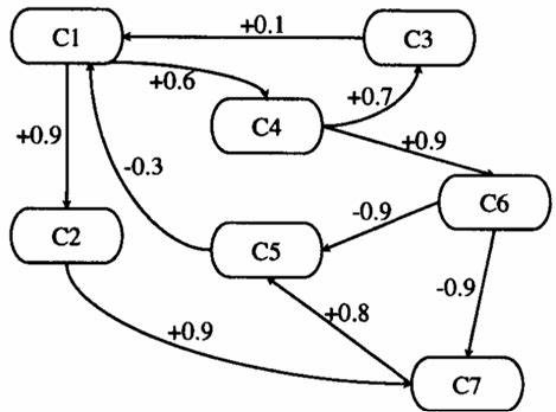
\includegraphics{Graphics/fcm_example.png}
    \caption{Ejemplo de un FCM}
\end{figure}

En esta imagen los $C_{i}$ hacen referencia al concepto $i$ del agente. El valor de los conceptos de los agentes se 
calcula en el momento en que este deba realizar una acción utilizando la siguiente función:
\begin{center}
    $X_{i}$(t+1) = F($X_{i}$(t) + $\sum_{j=1}^{n}${($X_{j}$(t) $\times$ $w_{j,i}$)})
\end{center}

donde $X_{i} (t)$ es el valor del i-ésimo concepto en el t-ésimo instante de tiempo, $i,j$=1, 2, ..., $n$, donde $n$ es el número
de conceptos, $w(i,j)$ es el peso que representa la relación que posee el concepto $i$ con el concepto $j$ y $F(x)$ es la función 
de transformación sigmoidal que normaliza los valores conceptuales al rango $[0,1]$. \autocite{Poczeta2020}

Existen varias formas y ejemplos en los cuales se puede utilizar un FCM, Nachazel en \autocite{Nachazel2021}
explica una nueva modificación a los FCM para la autonomía de decisión de los agentes. Propone dividir los conceptos en 3 clases
diferentes; necesidades, actividades y estados; para así agregar características que ayuden a la toma de decisiones y las necesidades 
internas que puede tener un agente. Es una visión sorprendente sobre en que se basa una entidad
o agente para la toma de decisiones o realizar una acción. Sin embargo, es de considerar,que utilizando otras clases, se 
puede lograr una mejor adaptación del FCM al necesitado: percepciones, sentimientos, acciones.\\ 
Con estas tres nuevas clases se podría utilizar el conocimiento que tiene un agente sobre el medio que lo rodea ($\textbf{percepciones}$) y  
cómo este se siente con respecto a esto ($\textbf{sentimientos}$) para así decidir sobre que acción final realizaría ($\textbf{acciones}$).\\

Al enlazar los conceptos y modelos antes vistos, se obtendría un entorno en el cual convivirían los agentes, teniendo o no algún
tipo de relación entre ellos (Red Social); en este existirían localidades a las cuales los mismos podrían acceder (Red Social) y 
cada agente poseería su propio FCM de percepción, sentimientos y acciones para elegir qué realizar en cada momento.
\chapter{Modelación para la simulación de enfermedades transmitidas por vectores}\label{chapter:proposal}
\section{Vectores en la naturaleza}
Un vector es un organismo vivo, como un insecto o artrópodo, que puede transmitir un agente 
infeccioso, como un virus, una bacteria o un parásito, de un huésped infectado a un huésped 
susceptible. Los vectores pueden actuar como intermediarios en la transmisión de enfermedades, 
ya sea mecánicamente, a través de la contaminación de alimentos o superficies con el agente 
infeccioso, o biológicamente, cuando el agente infeccioso se replica y multiplica dentro del 
vector antes de ser transmitido a un nuevo huésped. Los vectores son una parte integral de la 
epidemiología de muchas enfermedades infecciosas y desempeñan un papel crucial en su mantenimiento 
y propagación.\autocite{Reisen2010}\\

Según la OMS, las enfermedades airborne (arthropod-borne) representan 17 por ciento del total de 
las enfermedades infecciosas en el mundo, con 1,000 millones de casos y un millón de defunciones 
anuales \autocite{OMS2020}. Los vectores biológicos más comunes son los insectos hematófagos que 
al alimentarse de la sangre de un portador infectado, ingieren microorganismos patógenos que 
posteriormente inoculan a otro individuo.\\

\textbf{Características generales de los vectores:}\autocite{OMS2020}
\begin{enumerate}
    \item Especies específicas: Los vectores suelen ser especies específicas de insectos, 
    artrópodos u otros organismos. Por ejemplo, los mosquitos, las garrapatas, las pulgas y los 
    flebótomos son ejemplos comunes de vectores. 
    \item Capacidad de transmitir enfermedades: Los vectores tienen la capacidad de transmitir 
    agentes patógenos, como virus, bacterias o parásitos, de un huésped infectado a un huésped 
    susceptible. Esto puede ocurrir a través de la picadura o el contacto con el vector.
    \item Dependencia de los huéspedes: Los vectores dependen de la sangre u otros recursos de 
    sus huéspedes para alimentarse y reproducirse. Por lo tanto, su presencia y actividad están 
    estrechamente relacionadas con la disponibilidad de los huéspedes adecuados.
\end{enumerate}
\subsection{Enfermedades Transmitidas por Vectores (ETV)}
Entre las ETV que han aumentado en las últimas décadas están el 
paludismo o malaria, la fiebre hemorrágica por dengue, la esquistosomiasis, la tripanosomiasis americana 
o enfermedad de Chagas, la tripanosomiasis africana o enfermedad del sueño, la leishmaniasis, la fiebre 
amarilla, la encefalitis japonesa, la fiebre por zika  y la fiebre por chikungunya. Otras ETV menos frecuentes 
son la borreliosis o enfermedad de  Lyme y la enfermedad por el  virus del oeste del Nilo.\autocite{Torres2020}\\

\begin{figure}[htb]
    \centering
    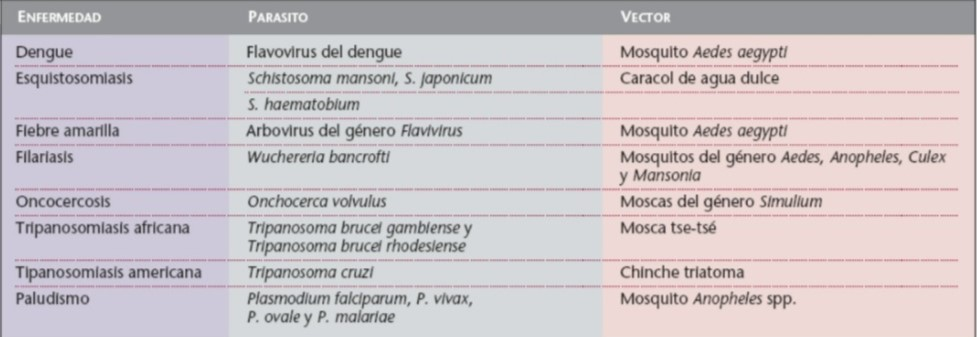
\includegraphics[width=1\textwidth]{Graphics/EnfVec.jpeg}
    \caption{Algunas enfermedades transmitidas por vectores.\autocite{Tercero2008}}
\end{figure}

La distribución de las ETV está vinculada a una serie de factores complejos 
de naturaleza demográfica, ecológica, medioambiental y social. Estos factores incluyen:
\begin{enumerate}
    \item El fenómeno del calentamiento global y el consiguiente cambio climático, que permite la adaptación de los vectores a nuevas altitudes y la propagación de patógenos en regiones previamente no afectadas.
    \item La sobrepoblación y el hacinamiento en áreas específicas, lo cual propicia un aumento en la presencia de vectores y hospederos susceptibles, como perros y gatos.
    \item La densidad de población de los artrópodos vectores y la diversidad de especies presentes en un área determinada.
    \item La falta de medidas adecuadas de higiene a nivel personal, en viviendas y en comunidades.
    \item El incremento en la frecuencia y distancia de los viajes internacionales.
    \item La existencia de marginación, pobreza y urbanización descontrolada.
\end{enumerate}

Actualmente, la enfermedad transmitida por vector con mayor crecimiento mundial es el dengue. 
Al igual que el virus del dengue, el del Zika, el chikungunya y la fiebre amarilla son transmitidos 
por los mosquitos Aedes aegypti y Aedes albopticus. Más de 3900 millones de personas en más de 129 
países corren el riesgo de contraer dengue, y se estima que cada año se registran 96 millones de casos 
sintomáticos y 40 000 muertes.\autocite{OMS2020}\\

\section{Dengue}
El dengue es una enfermedad viral transmitida por mosquitos que representa un desafío significativo 
para la salud pública a nivel mundial. Esta enfermedad se encuentra principalmente en regiones tropicales 
y subtropicales, pero su alcance se ha extendido durante las últimas décadas, llegando a afectar a más de 100 
países. El complejo del Dengue está formado por cuatro serotipos: dengue1, dengue2, dengue3 y dengue4. La 
infección humana por un serotipo produce inmunidad para toda la vida contra la reinfección por ese serotipo, 
pero el individuo queda susceptible a los otros tres. \autocite{Simmons2012} \\

Una vez una persona es picada por un mosquito infectado, se produce un período de incubación en esta, que puede 
durar de 5 a 7 días, luego de esto aparcen los primeros síntomas. El humano se encuentra enfermo aproximadamente
durante 7 o 15 días. En el momento en el que surgen los primeros síntomas comienza el período crítico de 
transmisión. Si en este intervalo de tiempo un mosquito pica a esa persona, entonces tiene una probabilidad 
alta de adquirir la enferemedad y luego de 8 a 12 días el virus se aloja en las glándulas salibales del mosquito
y es en esta etapa en que el mosquito es capaz de transmitir la enfermedad. \autocite{OMS2023} \\

Una de las características más preocupantes del Dengue es su capacidad para causar una amplia gama de síntomas, 
desde una fiebre leve hasta formas más preocupantes que pueden poner en peligro la vida. La forma grave de la 
enfermedad, conocida como fiebre hemorrágica del dengue, puede producir hemorragias internas, 
disfunción orgánica y shock. Esta forma afecta principalmente a niños pequeños, 
adultos mayores y personas con sistemas inmunológicos debilitados.\\

\textbf{Síntomas del Dengue:}\autocite{OMS2023}
\begin{enumerate}
    \item Fibre alta ($40^{\circ}$C).
    \item Dolores de cabeza.
    \item Dolor detrás de los ojos.
    \item Náuseas
    \item Vómitos
    \item Rash
\end{enumerate}

El mosquito aede aegypti es el vector del Dengue. El ciclo de vida de un mosquito es aproximadamente entre 4 y 
8 semanas y ocurre en varias etapas, huevo, larva, pupa y adulto. Los que transmiten la enfermedad son los mosquitos
hembras adultos. Estas necesitan de sangre para desarrollar los huevos y pueden volar hasta 3 kilómetros con 
el objetivo de encontrar un lugar para ponerlos, aunque no se espera que vuelen más de 100 metros del citio 
donde viven.\\

\section{Modelación del entorno}
Lo primero que se debe crear y modelar para simular como ocurre la propagación de enfermedades es el 
entorno en que ocurrirá la misma. La idea de este trabajo es lograr representar la realidad de la sociedad
y para esto se entiende que existen parámetros a desarrollar: las relaciones personales, los lugares y el comportamiento
de las personas.\\

\subsection{Loaclizaciones}
En la actualidad la mayoría de las personas tienen un programa de vida definido, es decir, una persona $x$ tiene una 
vivienda, un centro de trabajo y otros lugares a los que asiste por determinadas circunstancias; por lo que
para representar la sociedad, es necesario según se entiende, modelar estos lugares.\\

Para esto, los lugares son considerados un objeto en nuestro proyecto. Se entiende por lugar una localización en
la cual pueden asistir personas y vectores y además este puede brindar cierto recurso. Por ejemplo: ¿cómo se
representaría un mercado en nuestra simulación?, un mercado posee una capacidad para albergar personas y vectores 
y además brinda la posibilidad de obtener comida, aseo, entre otros.\\

\textbf{Localizaciones relevantes a representar:}
\begin{enumerate}
    \item Casas: representa un hogar familiar.
    \item Hospitales: indica un centro de atención médica.
    \item Centros de trabajo: hace referencia a todo lugar laboral, pero no significa que si una persona está en este, se encuentra trabajando, por ejemplo: en una escuela (centro de trabajo) hay personas que no están trabajando como los niños.
    \item Mercados.
\end{enumerate}

Este tipo de localizaciones nos permite abarcar toda construcción en la que pueden relacionarce las personas, pués
el tipo de lugar $"Centro$ $de$ $Trabajo"$ sirve de comodín en nuestra simulación.\\

\subsection{Personas}
Una de las herramientas conocidas para describir relaciones entre agentes son los grafos \autocite{Newman2003}. Un grafo
es un par ordenado $G = (V,E)$ donde $V$ es un conjunto no vacío de nodos y $E$ es un conjunto de pares 
no ordenados de aristas.\\

\begin{center}
    $G=(V,E)$ tal que:\\
    \begin{enumerate}
        \item $V$ = $\lbrace$ $v_{1}$, $v_{2}$, $v_{3}$, ..., $v_{n}$ $\rbrace$ es un conjunto finito de vértices.
        \item $E$ = $\lbrace$($v_{i}$,$v_{j}$)|$v_{i}$, $v_{j}$ $\in$ $V$ $\rbrace$  es un conjunto de pares no ordenados de vértices que representan las aristas del grafo.
    \end{enumerate}
\end{center}

En nuestro proyecto se construye un grafo que representa la relación ser familia y la relación conocidos, brindando
la posibilidad de escoger la probabilidad con la que se genere una arista entre dos nodos y la cantidad de nodos a crear. 
En este, un nodo $v_{i}$ representa a la persona $i$ de la simulación y una arista ($v_{i}$, $v_{j}$) simboliza,
o bien la relación $i$ $\rightarrow$ $j$ son familiares, o son conocidos, es decir no existe un tipo de arista para cada
tipo de relación. ¿Cómo se identifica entonces si la arista ($v_{i}$, $v_{j}$) representa la relación 
ser familia o la relación conocidos?\\

Para esto se realiza un proceso estocástico que ocurre una sola vez (al inicio de la simulación), el cual consiste 
en escoger de manera aleatoria el conjunto $C$ que se define a continuación.
\begin{center}
    Sea $G = (V,E)$ un grafo de nuestra simulación.\\
    Sea $H \subset V$ tal que $v_{i} \in H \Leftrightarrow \forall v_{j} \in H, (v_{i},v_{j}) \in E$\\
    Sea $C = \lbrace H_{1}, H_{2}, ..., H_{l} \rbrace$,$\forall i$ $H_{i} \subset V$ tal que si $v_{j} \in H_{i} \Rightarrow v_{j} \notin H_{k}$ $\forall k \neq i$\\
\end{center}

Teniendo esto en cuenta entonces las relaciones están definidas de la siguiente forma:
\begin{center}
    $\forall i,j$ $(v_{i}, v_{j}) \in E$ representa la relación ser familia  $\Leftrightarrow \exists k$ tal que $v_{i}, v_{j} \in H_{k}$, $H_{k} \in C$.\\
    Si $v_{i} \in H_{k}, v_{j} \notin H_{k}$, $H_{k} \in C$ y $\exists (v_{i}, v_{j}) \Rightarrow$ la arista $(v_{i}, v_{j})$  representa
    la relación ser conocidos.
\end{center}


\begin{figure}[htb]
    \centering
    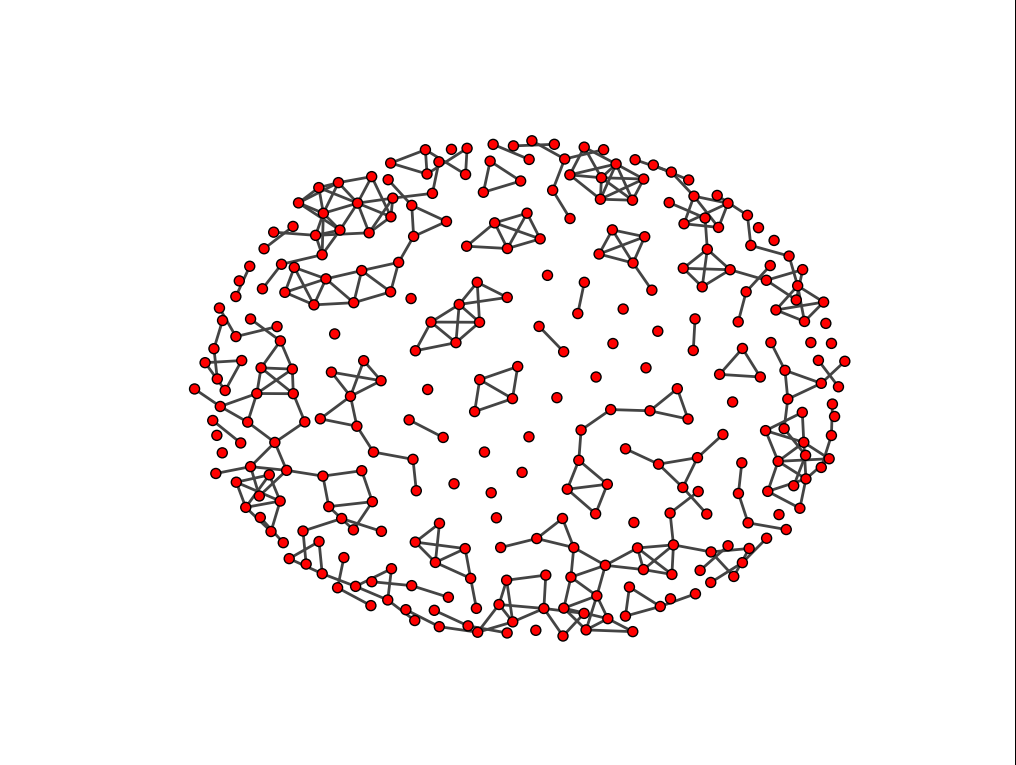
\includegraphics[width=0.8\textwidth]{Graphics/Grafo_Pers.png}
    \caption{Ejemplo de grafo de relaciones personales generados por el modelo. Personas: 300, probabilidad de arista: 0.05}
\end{figure}

\begin{figure}
    \centering
    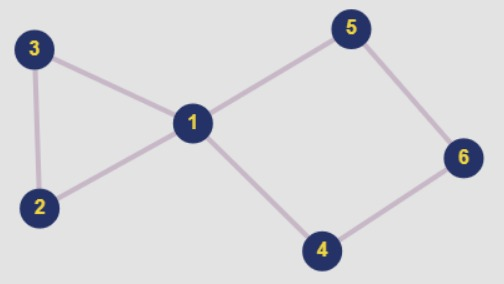
\includegraphics[width=0.3\textwidth]{Graphics/Grafo_Familias.jpeg}
    \caption{Ejemplo de grafo de relaciones personales para ilustrar.}
\end{figure}

En la figura 2.3 se observa un posible grafo generado. En este grafo los posibles conjuntos $H$ serían: 
$H_{1} = (1,2)$; $H_{2}=(1,3)$;$H_{3}=(2,3)$; $H_{4} = (1,2,3)$; $H_{5} = (1,5)$; $H_{6}=(1,4)$; $H_{7} = (4,6)$; $H_{8} = (5,6)$ y por último tantos conjuntos $H$ como nodos haya, es decir
todos los posibles cliques del grafo. De estos conjuntos se seleccionarían aleatoriamente algunos para formar el conjunto $C$;
por ejemplo $C = \lbrace H_{4}, H_{7}, H_{15} \rbrace$; y los nodos que estan en los $H_{i} \in C$ serían considerados
familias entre ellos.\\

Las personas, en el curso de la realización de sus actividades diarias (como el trabajo, el estudio o las compras),
se desplazan entre varios lugares, exponiéndose a agentes infecciosos dentro de estos lugares y transportando las
enfermedades. Para lograr representar y modelar estos procesos se genera una red de contactos sociales que puede
ser vista como un grafo bipartito, en el cual el conjunto $A$ está compuesto por todas las personas de la simulación
y el conjunto $B$ por todas las localizaciones. Las aristas en este grafo son dirigidas y representan 
el lugar en donde se encuentra la persona.\\
\begin{center}
    Sea $G = (V,E)$ grafo dirigido. 
    $\forall i,j$ si $(v_i,v_j) \in E \Rightarrow$ la persona $v_i$ se encuentra en el lugar $v_j$ 
\end{center}


\begin{figure}[htb]
    \centering
    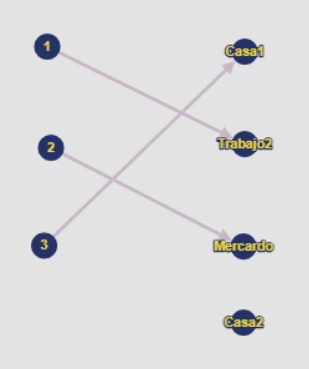
\includegraphics[width=0.3\textwidth]{Graphics/Grafo_Loc_Pers.jpeg}
    \caption{Ejemplo de grafo que representa a la red de contactos sociales.}
\end{figure}

El grafo definido anteriormente es un grafo dinámico, es decir este varía en dependencia del lugar en donde se encuentre
una persona, pues al decidir un agente ir a otro lugar, se elimina la arista que antes este tenía en el grafo y se 
añade la nueva arista, la cual representa el lugar en donde se encuentra en el momento. (Los vértices que representan
personas tienen $outdegree$ igual a 1)\\

\subsection{Vectores}
Los vectores son seres vivos al igual que las personas, pero a diferencia de estas estos poseen menos movilidad que las
personas. Para la representación de los vectores en el modelo no se tiene en cuenta la relación que 
poseen entre ellos pues se entiende que es suficiente con las relaciones de las personas para lograr simular 
la propagación de una enfermedad.\\ 

Los mosquitos como bien se mencionó anteriormente se establecen en un lugar y poco o nada se mueven de 
sus alrededores, por tanto, se decidió que los vectores en nuestra simulación no tuviesen la capacidad de moverse por
las localizaciones como las personas ya que esto nos acerca más a lo que ocurre en la realidad.\\

Los vectores se modelan con la posibilidad de morder y de infectarse. Estos según mecanismos estocástico
deciden si picar o no y teniendo en cuenta el nivel de infección de la persona y la susceptibilidad del mismo este
se infecta o no. También poseen un parámetro que representa la probabilidad de infectarse debido a una mordida, mientras
más alto más probable que este se infecte si pica o muerde a una persona enferma.\\

\begin{figure}[htb]
    \centering
    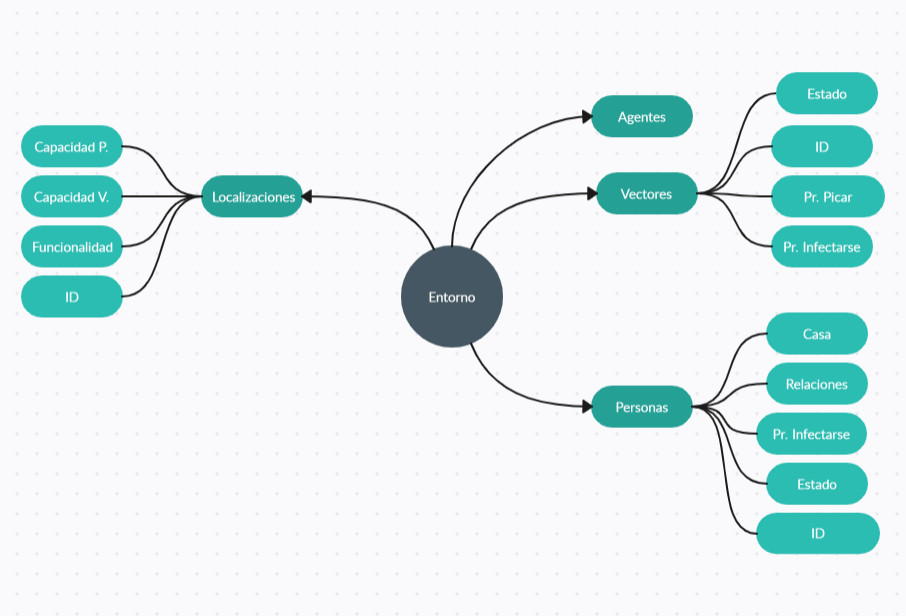
\includegraphics[width=0.9\textwidth]{Graphics/Pers_Loc_Vec.png}
    \caption{Esquema que representa el entorno modelado.}
\end{figure}
En la figura 2.4 se observa como se encuentra modelado el entorno de la simulación. Existen unos agentes que son las
personas y los vectores, los cuales poseen ciertas características y estos interactúan con las localizaciones para
cumplir sus propósitos; el de las personas trabajar y socializar y el de los vectores alimentarse, logrando así
acercarnos a un modelo que representa de forma precisa como se propaga un efermedad transmitida por vectores.

\section{Interacción de los agentes con el entorno}
Una vez diseñado el entorno y los agentes que conviven en el mismo, se abre paso al siguiente aspecto:
como interactúan entre sí. La interacción entre los agentes y su medio es esencial para comprender 
cómo se desarrollará y evolucionará el sistema en cuestión.\\
Existen muchas formas de desarrollar las interacciones, dependiendo del contexto y los objetivos establecidos
para los agentes. Pueden ser directas, donde los agentes interactúan entre sí de manera mutuamente perceptible,
indirectas, donde los agentes influyen en el entorno, y a su vez, el entorno afecta a la forma en que estos se 
comportan y un híbrido en el que los agentes según sus decisiones afectan al medio y a otros agentes, y también, 
el entorno los afecta.\\
Las interacciones pueden estar basadas en reglas predefinidas, donde se establecen normas, objetivos y una serie
de comportamientos específicos, o pueden ser adaptativas, donde los agentes aprenden a medida que intercambian con
el entorno, obteniendo retroalimentación del mismo, para modificar su comportamiento.\\
Una herramienta computacional que brinda la posibilidad de crear agentes con cierta inteligencia para manejar
sus decisiones son los Mapas Cognitivos Difusos (FCM). Para el diseño de un $FCM$ es necesario definir los 
conceptos que este agrupará, así como las categorías de conceptos.\\
¿Qué son los conjuntos difusos? Zadeh en \autocite{Zadeh1965} da respuesta a esta interrogante de la siguiente forma.
\begin{center}
    Sea $X$ un espacio de puntos en los que los elementos de $X$ son $x$. $X = \lbrace x \rbrace$
\end{center}
Un conjunto difuso $A$ en $X$ es caracterizado por una función de membresía $f_A(x)$ que asocia a cada punto en 
$X$ un valor real en el intervalo $[0, 1]$ con el valor de $f_A(x)$ en $x$ representando el 
grado de membresía de $x$ en $A$, tal que mientras más cerca el valor de $f_A(x)$ a la unidad más alto es 
el grado de membresía de $x$ en $A$. Pongamos un ejemplo representado en \autocite{Zadeh1965}.\\
Sea $X$ el conjunto de los números reales $R$ y sea $A$ un conjunto difuso de los números que son mucho mayores que 1.
La función $f_A(X)$ podría tener ciertos valores representativos como: $f_A(0) = 0$, $f_A(1) = 0$,
$f_A(5) = 0.01$, $f_A(10) = 0.2$, $f_A(100) = 0.95$, $f_A(500) = 1$.\\

Es importante notar que cuando el conjunto $X$ es un conjunto contable la función de membresía es parecida a una 
función de probabilidad (o parecido a la función de densidad cuando $X$ es continuo), evidentemente existen
diferencias entre estos conceptos las cuales son especificadas por Zadeh en \autocite{Zadeh1965}.\\

% \textbf{Algunas definiciones de conjuntos difusos:}\autocite{Zadeh1965}\\
% \begin{itemize}
%     \item Se dice que dos conjuntos difusos $A$ y $B$ son iguales, $\Leftrightarrow$ $f_A(X) = f_B(x)$ $\forall x$ en $X$.
%     \item Un conjunto difuso $A$ es vacío $\Leftrightarrow$ $f_A(x) = 0$ $\forall x$ en $X$.
%     \item El complemento de un conjunto difuso $A$ es $A'$ y es definido de la siguiente forma: $f_{A'} = 1 - f_A$.
%     \item $A \subset B \Leftrightarrow f_A \leqq f_B$
% \end{itemize}

En el Capítulo $"Estado$ $del$ $Arte"$ se realiza un acercamiento a la posibilidad de crear un $FCM$ con tres clases de 
conceptos; $Perspectiva$, $Sentimientos$ y $Acciones$. Cada clase tiene una serie de conceptos que posibilitan la 
interacción entre clases.\\
Al separar los conceptos se comienza a ver el grafo del $FCM$ como un grafo bipartito, en el cual el conjunto $A$
se encuentra formado por los conceptos de las clases $Perspectiva$ y $Acciones$ y el conjunto $B$ por la clase
$Sentimientos$. Entonces surge una interrogante, ¿cuál sería el flujo a seguir de este $FCM$ para que los agentes
decidan una acción u otra?.\\
La idea es la siguiente, un agente percibe un estado del entorno, este estado, provoca un sentimiento en el agente
y, a su vez, este sentimiento provoca una acción.
\begin{center}
    $Perspectiva \rightarrow Sentimientos \rightarrow Acciones$\\
\end{center}

A medida que va cambiando el entorno, va cambiando la perspectiva del agente esta afecta a los sentimientos del mismo 
y con esto cambia la probabilidad de efectuar una acción u otra. Por tanto, el tipo de relación utilizada en este $FCM$
es híbrida, cada pequeño cambio, ya sea, en el entorno, o en el mapa cognitivo difuso de un agente, afecta al $FCM$ de los
agentes restantes.\\

\subsection{Conceptos (Personas)}
\subsubsection{Perspectiva}
Para la sección de los conceptos de percepción se observa que una idea útil es que, para cada concepto, crear su contrapuesto
como concepto, por ejemplo, si se definiese el concepto $"cercanía de hospital"$, entonces sería útil definir el concepto
$"lejanía de hospital"$ pués las posibles acciones a ejecutar se beneficiarían por uno y se perjudicarían por el otro,
añadiendo facilidad a la decisión del agente.\\
\\
\textbf{Conceptos definidos para la categoría Perspectiva:}
\begin{itemize}
    \item Personas enfermas alta. (1.4)
    \item Personas enfermas baja. (1.4)
    \item Comida alta. (1.5)
    \item Comida baja. (1.5)
    \item Energía alta. (3)
    \item Energía baja. (3)
    \item Dinero alto. (1.5)
    \item Dinero bajo. (1.5)
    \item Enfermedad alta. (3.2)
    \item Enfermedad baja. (3.2)
\end{itemize}

Cada concepto en esta categoría, tiene un parámetro que representa cuan grande es el intervalo que se considera para darle un valor en la 
$fuziificación$ entre $(0,1)$ al concepto (el número que se encuentra entre paréntesis al lado del concepto), en caso 
de que sea menor o mayor a los límites del intervalo, su valor final es $0$ o $1$ respectivamente, pero, ¿por qué
se realiza este procedimiento?\\

La idea de implentar de esta forma esta categoría es para $fuzzificar$ teniendo en cuenta lo que se percibe 
del entorno. El valor de este parámetro por concepto nunca cambia, entonces surge la interrogante siguiente: 
¿cómo modelar que la perspectiva del entorno varía? Este valor pasa por un proceso en el cual se toman variables que si
cambian en el entorno y se utiliza el mismo para $fuzzificar$ el valor del concepto, el cual es distinto al parámetro 
representado en la lista anterior.\\

El proceso de $fuzzificación$ es distinto para cada concepto, pero por regla general se sigue la siguiente idea:\\
\begin{enumerate}
    \item Se toma un valor del entorno del entorno del agente que tenga relación con el concepto a $fuzzificar$, llamémosle $variable$ $de$ $fuzzificación$.
    \item Se obtiene un intervalo de valores utilizando el parámetro del concepto, llamémosle $intervalo$ $de$ $fuzzificación$.
    \item Se compara la $variable$ $de$ $fuzzificación$ con los extremos del $intervalo$ $de$ $fuzzificación$, en el caso de encontrarse incluida en este se decide si es más importante que este cerca del máximo o del mínimo del $intervalo$ $de$ $fuzzificación$ y se $fuzzifica$ de acuerdo al intervalo, teniendo en cuenta cual extremo es considerado $1$ y cual $0$ en el proceso de $fuzzificación$.
\end{enumerate}

\begin{center}
    Sea $v$ la $variable$ $de$ $fuzzificación$.\\
    Sea $(i_0, i_1)$ el $intervalo$ $de$ $fuzzificación$.\\
    Sea $r$ el resultado del proceso de $fuzzificación$.\\
    Sea $inv$ una variable booleana, tal que: $if$ $inv = True, v \geq i_1 \Rightarrow r = 1$ , $if$ $inv = False, v \leq i_0 \Rightarrow r = 1$\\
\end{center}
    Cuando $v$ se encuentra dentro del intervalo ocurre lo siguiente:
\begin{center}
    $if$ $inv = True$ $\Rightarrow$ $r = \frac{v - i_0}{i_1 - i_0}$\\
    $if$ $inv = False$ $\Rightarrow$ $r = \frac{i_1 - v}{i_1 - i_0}$
\end{center}

La combinación de valores en estos conceptos, o el valor de un concepto por sí mismo, afecta al valor que toma algún
concepto en la categoría $Sentimientos$.\\

\subsection{Sentimientos}
En esta categoría se tienen en cuenta los sentimientos básicos de un ser humano y los que mejor se adaptaban para
representar la movilidad de los mismos.\\
\\
\textbf{Conceptos definidos para la categoría Sentimientos:}
\begin{itemize}
    \item Miedo.
    \item Hambre.
    \item Necesidad.
    \item Enfermedad.
    \item Indiferencia.
    \item Cansancio.
\end{itemize}

\subsection{Acciones}
Se definen las acciones fundamentales que modelan el comportamiento de una persona en un ambiente epidémico.\\
\\
\textbf{Conceptos definidos para la categoría Acciones:}
\begin{itemize}
    \item Ir a trabajar.
    \item Ir al mercado.
    \item Ir al hospital.
    \item Caminar.
    \item Estudiar.
    \item Descansar.
    \item Prevenir.
\end{itemize}

Definamos ahora los conceptos que tienen relación entre sí, es decir que conceptos influyen en el valor de otros.
Para esto será necesario ilustrar en una imagen el grafo resultante.

% "people_sick_high" : (0, 1.4),
%             "people_sick_low" : (1, 1.4),
%             "food_high" : (2, 1.5),
%             "food_low" : (3, 1.5),
%             "energy_high" : (4, 3),
%             "energy_low" : (5, 3),
%             "money_high" : (6, 1.5),
%             "money_low" : (7, 1.5),
%             "sickness_high" : (8, 3.2),
%             "sickness_low" : (9, 3.2)

% "fear" : 10,
%             # "loneliness" : 11,
%             "hunger" : 12,
%             "necessity" : 13,
%             "disease" : 14,
%             "indifference" : 15,
%             "tiredness" : 16


% "go_to_work" : 17,
%             "go_to_market" : 18,
%             "go_to_hospital" : 19,
%             "go_around" : 20,
%             "study" : 21,
%             "rest" : 22,
%             "prevent": 23
\chapter{Detalles de Implementación y Experimentos}\label{chapter:implementation}


\backmatter

\begin{conclusions}
    Conclusiones
\end{conclusions}

\begin{recomendations}
    \textbf{Para trabajos futuros se propone:}
    \begin{enumerate}
        \item Construir un $FCM$ que modele las acciones que puedan realizar los mosquitos.
        \item Implementar un modelo de $Machine$ $Learning$\footnote{Aprendizaje de Máquina} utilizando redes neuronales que genere los valores de la matriz que representa al Mapa Cognitivo Difuso, con el objetivo de lograr modelar las acciones de las personas y mosquitos de una manera más precisa. El Mapa Cognitivo utilizado en la investigación ya se encuentra modelado como una red neuronal, cada categoría de conceptos se puede ver como una capa de la red, por lo que se recomienda implementarlo sobre la base del $FCM$.
        \item Añadir factores adicionales que influyen en la propagación de patógenos, como el clima, la reproducción ya sea de vectores o de personas, la edad de las personas, entre otros.
    \end{enumerate}
\end{recomendations}

\printbibliography[heading=bibintoc]


\end{document}